% ==============================================================================
% LAB 119
% UNDERSÖKNING AV RC-KRETS
% ------------------------
%
% Author:
% Jonas Sjöberg     <tel12jsg@student.hig.se>
% Oscar Wallberg    <tco13owg@student.hig.se>
%
% License:
% Creative Commons Attribution-NonCommercial-ShareAlike 4.0 International
% See LICENSE.md for full licensing information.
% ==============================================================================

\section{Uppmätning av Bode-diagram}\label{bode}

\subsection{Experimentuppställning}\label{}
% ------------------------------------------------------------------------------
En så kallad experimentplatta eller "breadboard" används för att konstruera
kretsen som illustreras i Figur \ref{bode-schema}.
\par För att generera en sinusformad signal används signalgeneratorn HP33120A,
vars utgång kopplas genom en BNC-förgrening till oscilloskopet Agilent 54621A
och genom en BNC- banankontaktadapter, med "banankablar" till
breadboardplattans skruvterminaler.
\par Oscilloskopet visar signalen från kretsens ingång, dvs signalgeneratorns
utgångs, på kanal ett. Kanal två kopplas till kretsens utgång, Punkt A i
\ref{bode-schema} med en oscilloskop-prob. Proben ställs till att dämpa
med en faktor av 10:1 och den vertikala skalan justeras en dekad nedåt, så att
båda kanalerna visas med samma skalfaktor.


\begin{figure}
    \centering
    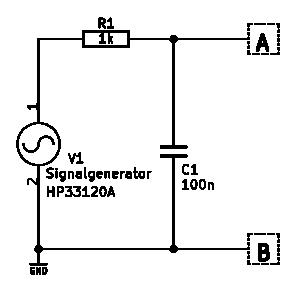
\includegraphics[width=0.6\linewidth]{img/1-freqdom_schem}
    \caption[Schematisk ritning av labbkoppling, första ordningens RC-filter.]
    {Schematisk ritning av labbkoppling, första ordningens RC-filter.}
    \label{bode-schema}
\end{figure}


\subsection{Mätresultat}\label{}
% ------------------------------------------------------------------------------
% TODO:

\subsection{Simulering}\label{}
% ------------------------------------------------------------------------------
Kretsen simuleras i \texttt{LTSpice} enligt Figur~\ref{fig:sim1}.

\begin{figure}
    \centering
    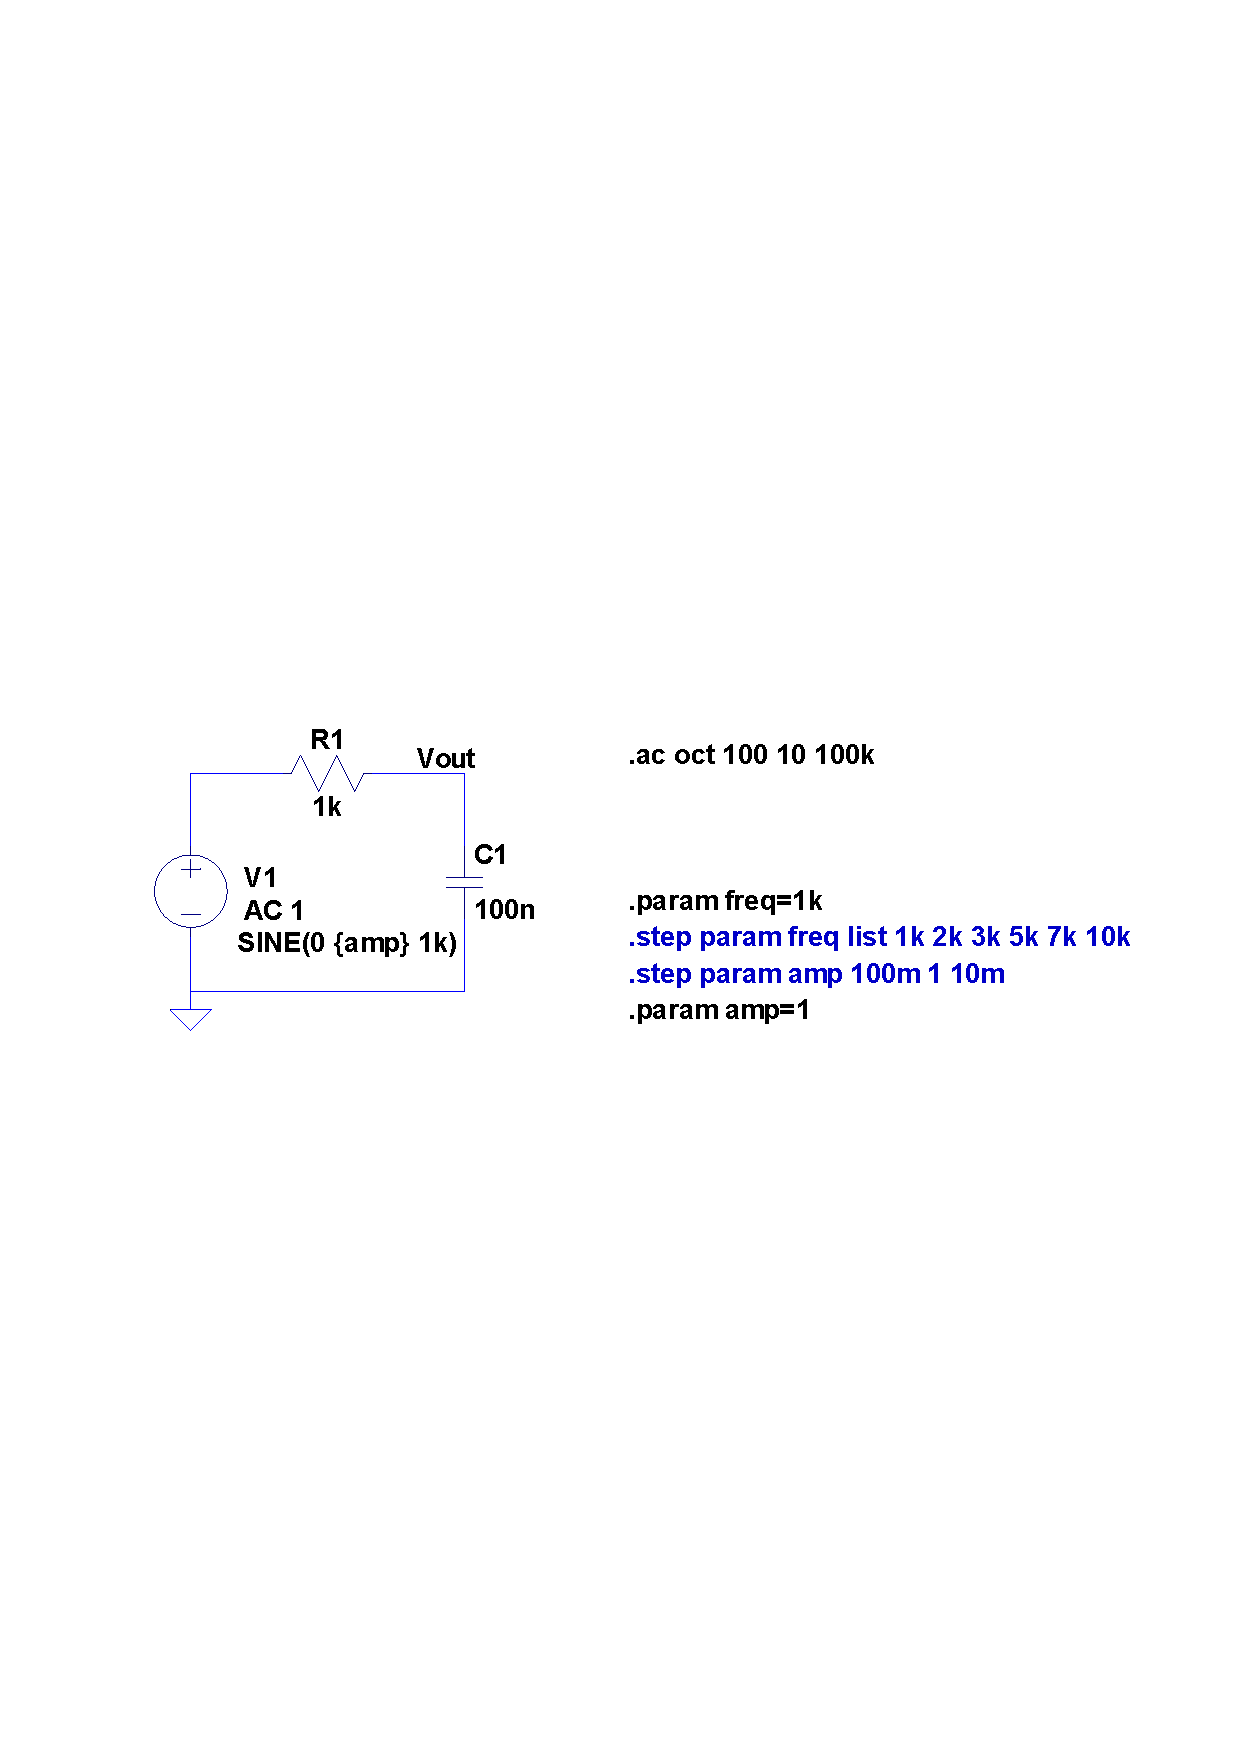
\includegraphics[width=0.6\linewidth]{sim_ltspice/lab4_1.pdf}
    \caption[Simulering av labbkopplingen i LTSpice.]
    {Simulering av labbkopplingen i LTSpice.}
    \label{bode-sim}
\end{figure}

\begin{sidewaysfigure}[ht]
    \centering
    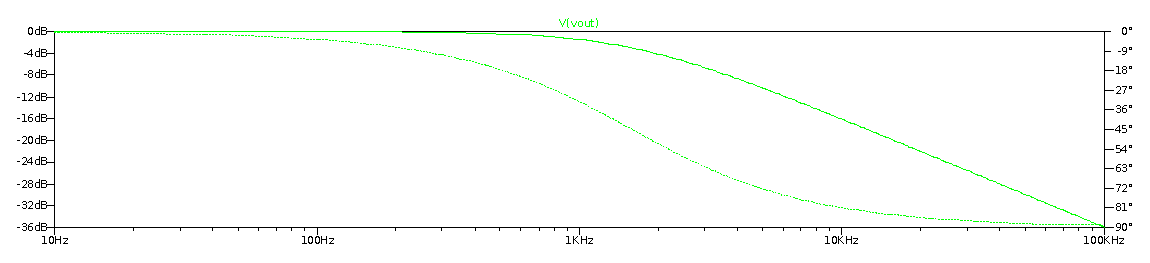
\includegraphics[\linewidth]{sim_ltspice/lab4_1-acplot.eps}
    \caption[Kretsens frekvensåtergivning. Resultat från simulering av
    labbkopplingen i LTSpice.]
    {Resultat från simulering av labbkopplingen i LTSpice.}
    \label{bode-sim}
\end{sidewaysfigure}

\begin{sidewaysfigure}[ht]
    \centering
    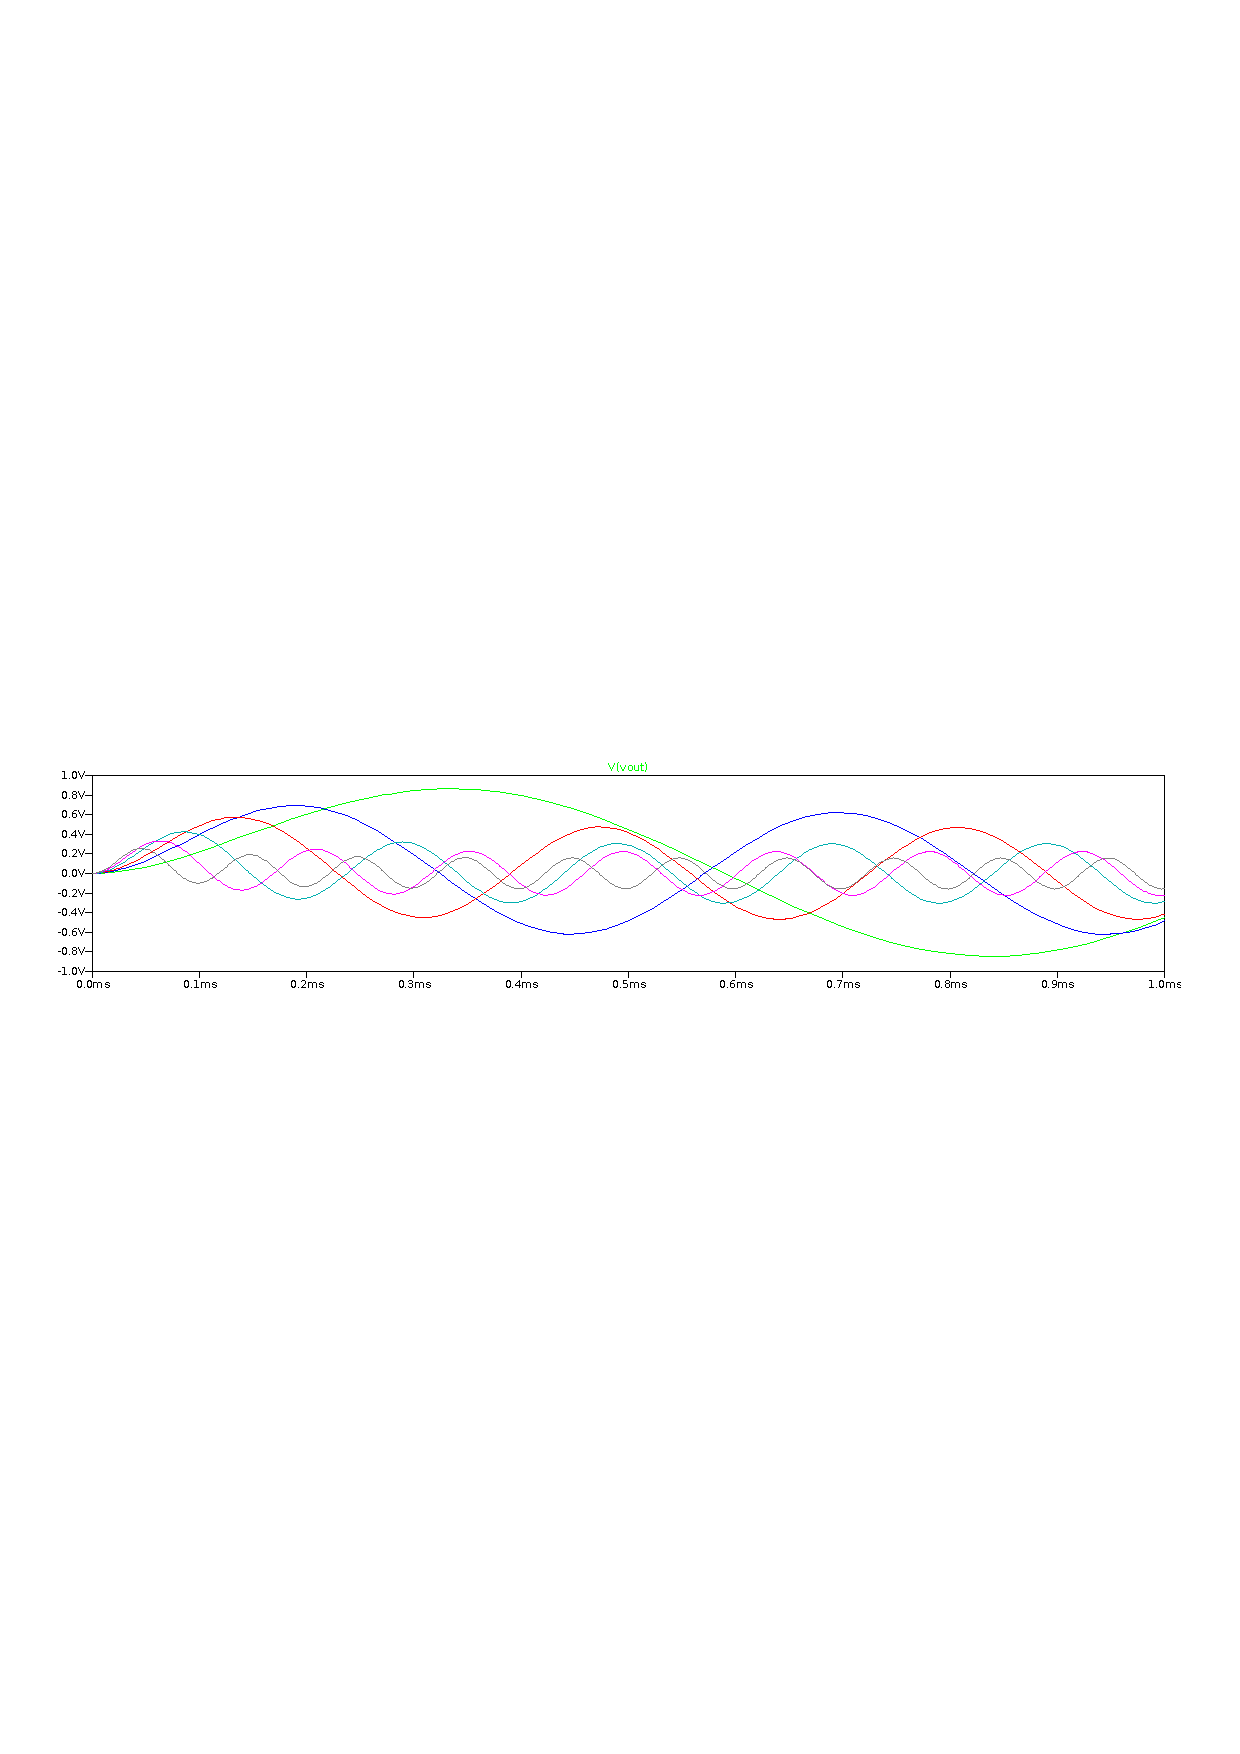
\includegraphics[\linewidth]{sim_ltspice/lab4_1-tranplot.pdf}
    \caption[Kretsens transientrespons för olika frekvenser hos V1. Resultat
från simulering av labbkopplingen i LTSpice.]
    {Resultat från simulering av labbkopplingen i LTSpice.}
    \label{bode-sim}
\end{sidewaysfigure}



\subsection{Kommentar}\label{}
% ------------------------------------------------------------------------------
% TODO:


